\chapter{La Business Intelligence e la Business Analytics}
\label{ch:Business Intelligence and Analytics}

\begin{citazione}
È un errore enorme teorizzare a vuoto. Senza accorgersene, si comincia a deformare i fatti per adattarli alle teorie, anziché il viceversa. Sherlock Holmes\cite{conan_doyle_cyte}
\end{citazione}

Come spiegato in precedenza, l'analisi dei dati è un termine "astratto" utilizzato per fare riferimento ad un processo di multiple azioni atte a gestire i dati e ricavarne informazioni. Di quest'ultima parte solitamente se ne occupa il mondo della business intelligence e della business analytics. Questi processi solitamente si interfacciano direttamente con il sistema di data warehouse predisposto dall'azienda (entrando in questo modo nel \textit{livello di presentazione} dello stesso).  

\section{La Business Intelligence}
In generale il termine Business Intelligence viene utilizzato per indicare:\cite{meauserement_of_bi}

\begin{itemize}
    \item Informazioni e conoscenze rilevanti che descrivono l'ambiente aziendale, l'organizzazione stessa e la sua situazione in relazione ai mercati, ai clienti, ai concorrenti e alle questioni economiche.
    \item Un processo organizzato e sistematico attraverso il quale le organizzazioni acquisiscono, analizzano e diffondono informazioni da fonti interne ed esterne significative per le loro attività commerciali e per il processo decisionale.
\end{itemize}

Più precisamente, la \textbf{Business Intelligence} (\textbf{BI}) si può definire come «un approccio attivo, basato su modelli e prospettico per scoprire e spiegare aspetti nascosti e rilevanti per le decisioni in grandi quantità di dati aziendali per informare meglio i processi decisionali aziendali».\cite{bi_strategic_intelligence}

\begin{comment}
\begin{figure}[!h]
    \centering
    
\includegraphics[width=0.75\linewidth]{figure//capitolo_4/Business Intelligence.jpg}
    \caption{La Business Intelligence}
    \label{fig:Business Intelligence}
\end{figure}
\end{comment}

Come abbiamo potuto vedere in precedenza, per i processi di analisi e gestione dei dati non esistono delle definizioni fisse che indichino quali processi, protocolli, modelli o infrastrutture siano necessari per poterli svolgere. In un mondo in cui la tecnologia è in continua evoluzione tali elementi cambiano con essa, differenziando inoltre da azienda ad azienda e da business a business a seconda delle situazioni e necessità. Per questo motivo si può generalizzare il concetto dicendo che «la business intelligence è essenzialmente una conoscenza del business tempestiva, accurata, di alto valore e perseguibile, nonché i processi di lavoro e le tecnologie utilizzate per ottenerla».\cite{bi_for_dummies}

Quindi, la BI è identificabile come il risultato finale e naturale dell'unione di diversi sistemi e processi, definiti precedentemente, atti a supportare il processo decisionale di un'azienda. L'emergere dell'uso di sistemi di data warehousing, i progressi svolti nella pulizia dei dati, le maggiori capacità di hardware e software e l'evoluzione delle tecnologie connesse ad Internet si combinano per creare un ambiente ricco ed utile per la business intelligence. Principalmente, la BI attinge informazioni da differenti sistemi.\cite{researchgate_bi_systems}

\begin{comment}
\begin{figure}[!h]
    \centering
    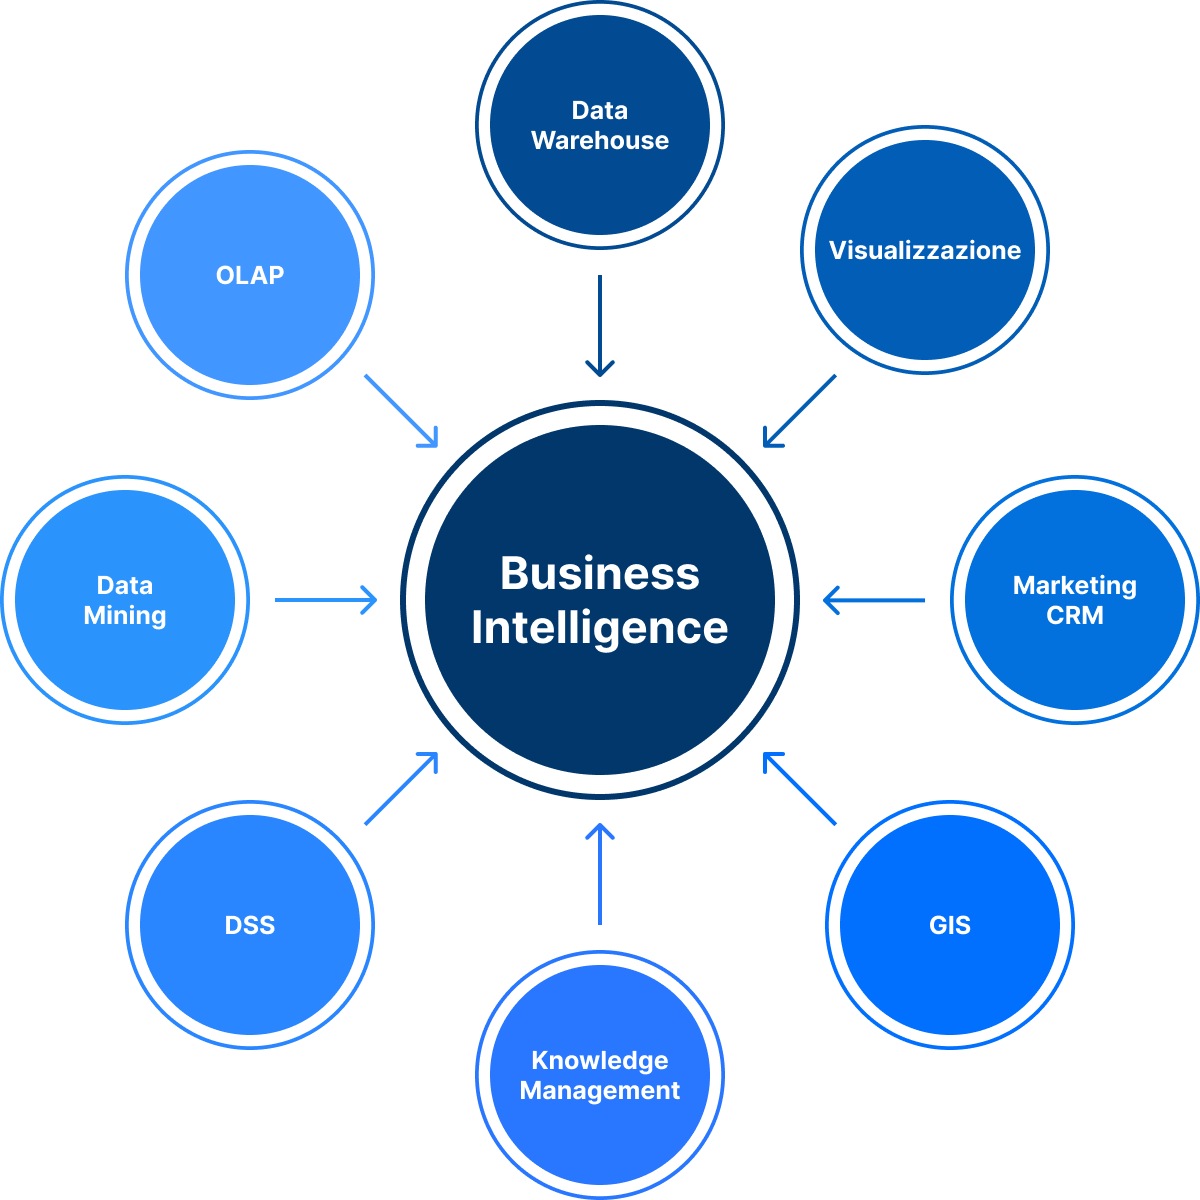
\includegraphics[width=0.5\linewidth]{figure//capitolo_4/Business Intelligence Systems.png}
    \caption{Sistemi di integrazione con la Business Intelligence}
    \label{fig:Business Intelligence Systems}
\end{figure}
\end{comment}

\subsection{La storia}

\subsubsection{L'origine}

Nel 1958 Hans Peter Luhn pubblica un proprio articolo dando vita al termine \textit{\textbf{Business Intelligence System}} (per questo ne è considerato il "padre"). Il ricercatore di IBM descrive l'idea dello sviluppo di un sistema automatizzato dedicato a diffondere le informazioni all'interno aree differenti della stessa organizzazione così da semplificarne l'interazione. Nell'articolo Luhn spiega anche l'ordine del nome dicendo: «Per "\textit{Business}" si intende un insieme di attività svolte per qualsiasi scopo, sia esso scientifico, tecnologico, commerciale, industriale, legale, governativo, di difesa, ecc. La struttura di comunicazione che serve alla conduzione di un'azienda può essere definita un "\textit{Intelligence System}". La nozione di "\textit{Intelligence}" è anche definita qui, in senso più generale, come "la capacità di comprendere le interrelazioni dei fatti presentati in modo tale da guidare l'azione verso un obiettivo desiderato"».\cite{luhn_business_intelligence}

\subsubsection{L'evoluzione}

Le attuali applicazioni di Business Intelligence sono soluzioni software, che permettono di svolgere calcoli e analisi sui dati, derivate da un evoluzione costante avvenuta negli anni. Di seguito sono riportati le varie fasi affrontate nel suo percorso storico (sotto forma di \textit{BI\&A}, ovvero \textit{Business Intelligence and Analytics}).\cite{researchgate_bi_and_ba}

\begin{enumerate}
    \item \textbf{BI\&A 1.0}: La gestione dei dati e la creazione dei sistemi di data warehouse sono considerate le fondamenta di questa fase. Non a caso essa si basa principalmente sulle tecniche di archiviazione, estrazione e ottimizzazione dei dati archiviati all'interno dei sistemi di gestione dei database relazionali dell'azienda. Questa prima fase fornisce le basi per l'analisi dei dati moderna e tecniche simili come query di database, elaborazione analitica online e strumenti di reporting standard.
    \item \textbf{BI\&A 2.0}: Con l'inizio del ventunesimo secolo Internet e le relative applicazioni Web hanno iniziato a generare enormi volumi di dati. Oltre ai dati normalmente loggati dai vari servizi, questi hanno iniziato a generare anche altre tipologie di dati non strutturati che permettessero di capire come gli utenti si interfacciassero al mondo del Web. Inoltre, con l'avvento dei social media la crescita dei dati ha aggravato la necessità di strumenti, tecnologie e tecniche che permettessero di svolgere un'analisi che permettesse di apprendere meglio le interazioni delle persone con questi servizi e tra di loro.
    \item \textbf{BI\&A 3.0}: Con il passare del tempo e l'avvento del IoT il numero di dispositivi mobili, di qualsiasi genere e per qualsiasi utilizzo (personale, casalingo, aziendale privato o pubblico), a disposizione della popolazione mondiale è in larga crescita. Poiché si prevede che lo sviluppo del Web 3.0 e del mondo interno ad esso non possa che continuare, la corsa all'estrazione delle informazioni significative e preziose da queste fonti di dati avrà un futuro altrettanto importante e prospero. Proprio per questo motivo tale periodo promette di avere interessanti risvolti dal punto di vista della ricerca e dello sviluppo sia in ambito accademico che industriale.
\end{enumerate}

% TODO: Aggiungere tabella rappresentate le fasi

\subsection{L'apporto della Business Intelligence}

\subsubsection{Il valore}

Dal punto di vista economico, il valore aziendale di un investimento è misurato come il valore attuale netto dei flussi di cassa dopo le imposte associate all'investimento in questione.\footnote{\textit{Il flusso di cassa al netto delle tasse} (\textit{CFAT}) è una misura della performance finanziaria che mostra la capacità di un'azienda di generare flussi di cassa (ovvero, la liquidità netta e gli equivalenti liquidi trasferiti dentro e fuori da un'azienda) attraverso le sue operazioni.\cite{cfat_definition}}
Allo stesso modo, un investimento nell'abito della Business Intelligence crea un bene che deve essere adoperato per generare CFAT incrementali, per far si che comporti aumento delle entrate, riduzione dei costi o entrambi. In altre parole, il valore aziendale della BI risiede nel suo utilizzo all'interno dei processi di gestione che influenzano i processi operativi che generano entrate o riducono costi, e/o nel suo utilizzo all'interno degli stessi processi operativi che lo adottano.\cite{decisionpath_bi_value}

% TODO: aggiungere immagine sulla BI, valore oppure benefici

\subsubsection{I benefici}

Nella gestione aziendale un efficiente accesso ai dati può costituire uno strumento di business in grado di migliorare l'efficacia dei processi decisionali, grazie soprattutto alla individuazione delle informazioni necessarie a perseguire uno dei principi che costituiscono il punto di forza per eccellenza, ovvero il miglioramento continuo. Nell'ottica di un costante processo di miglioramento può essere determinante l'individuazione dei possibili punti di forza e/o di debolezza del core business, oltre all'individuazione delle opportunità e delle vulnerabilità, definendo le linee guida e le istruzioni operative che solo da una analisi approfondita possono scaturire, grazie anche ad un approccio derivante da una pianificazione strategica aziendale consapevole.\cite{dalla_bi_al_dw}

Per questo motivo, le aziende hanno iniziato ad adoperare sistemi di Business Intelligence nei propri processi decisionali. Per comprendere meglio a cosa sia dovuto questo alto valore di ROI\footnote{Il \textit{Return Of Investment} (\textit{ROI}, o \textit{ritorno sull'investimento}) è una misura di performance utilizzata per valutare l'efficienza o la redditività di un investimento misurando direttamente l'ammontare del rendimento di un particolare investimento rispetto al suo costo.\cite{investopedia_roi}} di seguito sono riportati tutti i vantaggi ricavabili dall'uso della BI nella propria azienda.\cite{oracle_business_intelligence}

\begin{itemize}
    \item Migliorare l'accuratezza dei dati.
    \item Prendere decisioni migliori più rapidamente.
    \item Migliorare i risultati mission-critical.
    \item Condividere i dati tra aree funzionali aziendali.
    \item Ottenere una maggiore visibilità delle informazioni finanziarie e operative.
    \item Identificare e ridurre le inefficienze.
    \item Eliminare sprechi, frodi e abusi.
    \item Migliora la produttività e il morale dei lavoratori.
    \item Aumentare il ritorno sull'investimento riducendo il costo totale di proprietà.
    \item Migliorare la trasparenza e il servizio a tutti i livelli.
\end{itemize}

\subsubsection{I punti chiave che indicano la necessità di BI}

Di seguito sono riportati otto punti chiave che indicano la necessità da parte di un'azienda dell'adozione di una soluzione di Business Intellingence per migliorare la propria gestione.\cite{boomper_book_of_bi}

\begin{itemize}
    \item \textit{Difficoltà nell'accesso ai dati}. In settori competitivi, è essenziale che le aziende possano accedere rapidamente ai propri dati. Di conseguenza, è essenziale che i decision maker accedano a specifiche informazioni con facilità e immediatezza.
    \item \textit{Dati provenienti da diverse fonti}. Quando un'azienda raccoglie dati da varie fonti, consolidarli in informazioni utili può essere difficile (diversi dipartimenti possono adottare metodologie o formati differnti per il salvataggio e il reporting dei dati). La BI può contribuire a unificare questi dati.
    \item \textit{Dipendenza dai fogli di calcolo}. Utilizzare i fogli di calcolo come principale mezzo per archiviare le informazioni con l'aumentare dei volumi di dati e della loro complessità è un processo inefficiente, tedioso e complicato. Una soluzione di BI può contribuire a razionalizzare il processo di raccolta, analisi e reportistica dei dati.
    \item \textit{Blocchi nella reportistica}. In molte aziende, la business intelligence e la reportistica sono completamente di competenza del reparto \textit{IT}\footnote{Il termine \textit{IT} fa riferimento all'intero spettro di tecnologie per l'elaborazione delle informazioni (compresi software, hardware, tecnologie di comunicazione e servizi correlati). Generalmente, l'ambito dell'IT non include tecnologie integrate che non generano dati per uso aziendale.\cite{gartner_it}}. Ciò può creare blocchi nel processo di reportistica e ritardi che possono rendere obsolete le informazioni. Una soluzione di BI può contribuire a ridurre questi blocchi dando più potere alle persone attraverso la capacità di autogestire e creare i propri report senza la necessità di conoscenze o esperienza tecniche.
    \item \textit{I tuoi dati non forniscono insight attuabili}. Le aziende possono spesso focalizzarsi così tanto sul processo di raccolta dati che finiscono col trascurare l'importanza della produzione di \textit{insight}\footnote{Le \textit{insight}, o \textit{intuizioni}, sui dati sono le conoscenze che un'azienda ottiene analizzando insiemi di informazioni relative a un determinato argomento o situazione, fornendo in questo modo spunti che aiutano le aziende a prendere decisioni.\cite{datarobot_insight}} applicabili. Per questo motivo le aziende dovrebbero adottare un approccio basato sulla qualità piuttosto che sulla quantità dei dati (evitando di raccogliere semplicemente grandi quantità di informazioni prive di significato).
    \item \textit{Dati obsoleti}. Uno dei principali problemi che affligge le aziende è che i loro dati non sono aggiornati. Ciò potrebbe dipendere da ritardi nella raccolta, analisi o reportistica delle informazioni e può avere conseguenze negative sulle prestazioni aziendali. Una soluzione di BI può automatizzare l'elaborazione e la consegna dei dati, con molte soluzioni in grado di pianificare i report in anticipo, garantendo che i dirigenti aziendali dispongano sempre delle informazioni necessarie.
    \item \textit{Difficoltà nella visualizzazione dei dati}. La visualizzazione dei dati è una parte fondamentale della Business Intelligence, ma senza l'esistenza di una soluzione di BI, spesso viene trascurata. I dati una volta raccolti andrebbero sfruttati per essere definibili come utili.
    \item \textit{Impossibilità di accedere ai dati su dispositivi multipli}. Al giorno d'oggi, è sempre più importante che le informazioni siano accessibili in qualunque momento e luogo. Per questo motivo nuovi strumenti di BI sono indirizzati verso un approccio che permetta di utilizzarli da dispositivi multipli.
\end{itemize}

\subsection{Il framework per la BI}
La Business Intelligence, come accennato in precedenza, essendo una branca dell'analisi dati comprende diversi aspetti precedentemente accennati e li racchiude in un unico processo. Per questo motivo, è possibile suddividere il framework di BI in tre differenti componenti:\cite{academiaedu_bi_integrated_approach}

\begin{enumerate}
    \item \textit{Acquisizione}. Tale componente, il più "profondo", si occupa della prima parte del data warehousing, ovvero la raccolta dati associati. Tale fase di acquisizione viene svolta applicando il processo di ETL.
    \item \textit{Archiviazione}. Tale componente si occupa di memorizzare i dati preprocessati dal componente di acquisizione nel data warehouse (e nei relativi data mart se il DW li utilizza) con i relativi metadati.
    \item \textit{Accesso e Analisi}. Tale componente, il più "esterno", possiede strumenti e tecniche di accesso che forniscono all'utente finale un accesso diretto e interattivo con i dati salvati. Tale interfaccia permette di svolgere in modo intuitivo e semplice tutti i processi di interrogazione, reportistica e visualizzazione dei dati che si necessita di analizzare.
\end{enumerate}

\begin{comment}
\begin{figure}
    \centering
    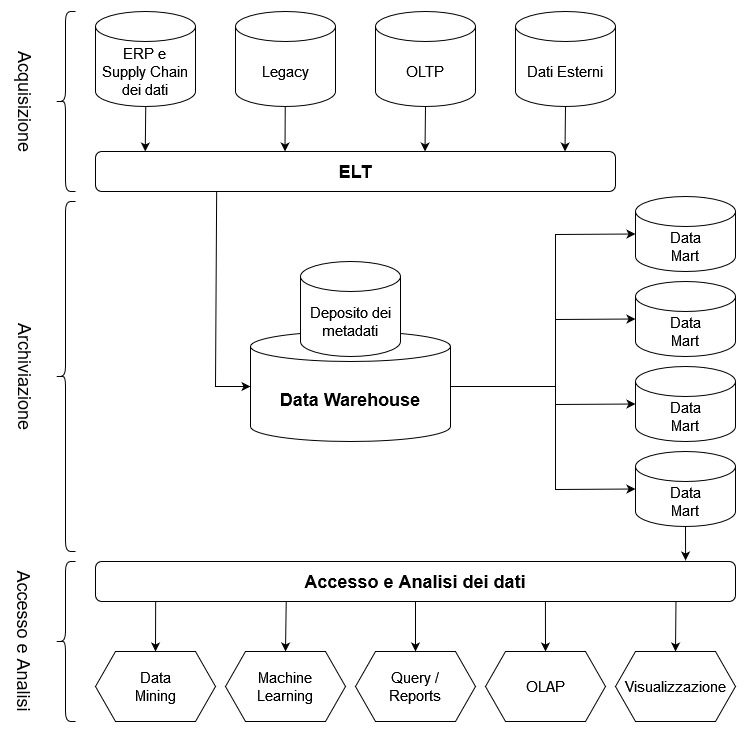
\includegraphics[width=0.5\linewidth]{figure//capitolo_4/Business Intelligence Framework.jpg}
    \caption{Il framework della Business Intelligence}
    \label{fig:Business Intelligence Framework}
\end{figure}
\end{comment}

\subsection{Sviluppo di una soluzione aziendale}

\subsubsection{Processo ciclico}
Un processo di Business Intelligence, per quanto possa differire per approccio, l'argomento e lo scopo di riferimento, in generale è caratterizzato da alcuni passaggi fondamentali per la sua implementazione, ovvero:\cite{citeseerx_bi_process} 

\begin{enumerate}
    \item \textit{Analisi}. Prima di essere predisposto per l'utilizzo, è necessario svolgere un'analisi dei requisiti che indichi quali sono i KPI\footnote{Un indicatore chiave di prestazioni (\textit{Key Performance Indicator}, o \textit{KPI}) si riferisce ad una misurazione quantificabile utilizzata per valutare le prestazioni a lungo termine di un'azienda rispetto a quello specifico ambito di interesse, aiutando a determinare i risultati strategici, finanziari e operativi di una compagnia (potendo anche metterli a paragone con altri competitor dello stesso settore).\cite{investopedia_kpi}} richiesti dagli utenti finali. Tale fase permette di identificare, ad alto livello,i vari componenti che una possibile soluzione dovrebbe integrare.
    \item \textit{Progettazione}. Sulla base dei requisiti stilati nella fase precedente, in questa vengono identificate specificatamente quali tecnologie siano appropriate per rendere reale la soluzione precedentemente ideata.
    \item \textit{Sviluppo}. Questa fase comporta la messa in atto di tutti i processi studiati, delle infrastrutture progettate e dei modelli di analisi scelti. L'implementazione, inoltre, dipende spesso anche dalla tipologia di dati che dovranno essere gestiti dal sistema, poiché ognuno può necessitare di funzionalità differenti.
    \item \textit{Distribuzione}. Una volta implementata e testata, la soluzione viene messa a disposizione degli utenti finali. Sono proprio quest'ultimi le persone da cui dipende la riuscita finale del progetto, poiché tale fase include lo sviluppo di report e analisi predefinite per i decision maker aziendali.
    \item \textit{Evoluzione}. Tale fase si può dire che è ciò che rende ciclico l'intero processo appena esplicato. Questo perché bisogna sempre valutare il successo del sistema creato per poi estenderlo con ulteriori funzionalità e anche modificare, ottimizzare e rivalutare scelte fatte in precedenza.
\end{enumerate}

\begin{comment}
\begin{figure}
    \centering
    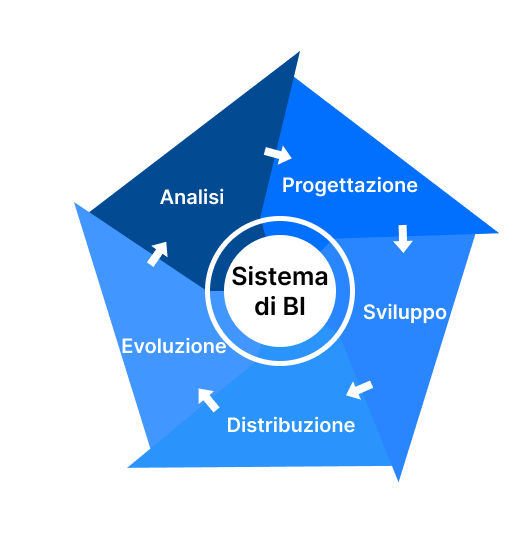
\includegraphics[width=0.75\linewidth]{figure//capitolo_4/Business Intelligence Life Cycle.png}
    \caption{Ciclo di vita di un processo di Business Intelligence}
    \label{fig:Business Intelligence Life Cycle}
\end{figure}
\end{comment}

\subsubsection{Modello approfondito}

In modo più approfondito, l'implementazione di un sistema di Business Intelligence si compone di 8 fasi differenti:\cite{altexsoft_bi_implementation}

\begin{enumerate}
    \item \textit{Introduzione della BI ai dipendenti e agli stackholder}. Per poter sfruttare a pieno un sistema di BI è necessario far apprendere a tutti gli stakeholder\footnote{Uno \textit{stakeholder} è una parte (individuo, gruppo o organizzazione) che ha interesse in un'azienda e può influenzare o essere influenzata dalle sue attività (ad esempio, investitori, dipendenti, clienti o fornitori).\cite{investopedia_stakeholder}} le sue possibili funzionalità ed obiettivi. A seguito di una prima spiegazione, è poi necessario identificare il problema che si vuole risolvere o analizzare.
    \item \textit{Definizione di obiettivi, KPI e requisiti}. Una volta identificato il problema che si vuole affrontare, è necessario definire quali sono gli obiettivi che si vogliono raggiungere e quali possono essere (ipoteticamente parlando) dei KPI e metriche di valutazione rilevanti nell'ambito di interesse (possono essere sia vincoli finanziari che indici di prestazione). Ciò permetterà di comprendere anche quali sono i requisiti necessari allo sviluppo ed utilizzo della soluzione ricercata.
    \item \textit{Scelta degli strumenti o di una soluzione personalizzata}. A seguito della definizione dei requisiti è possibile comprendere quale soluzione possa essere la migliore da adoperare nel proprio sistema. Esistono molte soluzioni, tuttavia una soluzione personalizzata ad hoc per un'azienda può essere la scelta più adatta. Per comprendere quale sia la soluzione più conveniente è necessario svolgere una ricerca di mercato che permetta di mettere a paragone tutte le possibili scelte.
    \item \textit{Definizione di un team predisposto}. Per poter sfruttare al meglio un sistema del genere spesso è necessario definire un team predisposto a tale compito. Solitamente si cerca di inserire nel team personale di differenti reparti in modo da avere un possibile contatto diretto con gli stessi e personale conoscente del proprio ambito di lavoro. Inoltre, l'eterogeneità del gruppo permetterà una possibile evoluzione dello stesso grazie a punti di vista e pensieri differenti.
    \item \textit{Documentazione della strategia adottata}. Per creare un sistema nel modo corretto e senza errori, all'interno del progetto in questione viene adottata una specifica strategia. Tale strategia può includere differenti componenti, per questo motivo è importante riportare una documentazione che spieghi per ognuno di essi l'approccio adottato a riguardo. Ciò permette di semplificare la manutenibilità del sistema stesso.
    \item \textit{Configurazione di strumenti di integrazione e data warehouse e scelta di un approccio architetturale}. Tale fase dipende molto dallo strumento adottato, una scelta personalizzata o una plug and play avranno impatti differenti sulla difficoltà e capacità di integrazione con le infrastrutture e software dell'azienda.
    \item \textit{Implementazione di un'interfaccia utente finale}. In questa fase i dati vengono modellati, gestiti e infine messi a disposizione degli utenti finali grazie ad un'apposita interfaccia degli strumenti di BI. La creazione di corretti report è una fase essenziale e critica dell'intero processo perché permette l'analisi e la comprensione delle informazioni necessarie a prendere decisioni basate su tutti i dati gestiti dal sistema.
    \item \textit{Formazione degli utenti finali}. Un'ulteriore fase che può essere affrontata è la formazione degli utenti finali in modo da agevolare l'interazione e integrazione degli strumenti nei normali processi di gestione e sviluppo del personale aziendale. In caso contrario, si potrebbe riscontrare un problema di un utilizzo scorretto o sbagliato da parte degli utenti dello strumento messo a disposizione.
\end{enumerate}

\begin{comment}
\begin{figure}
    \centering
    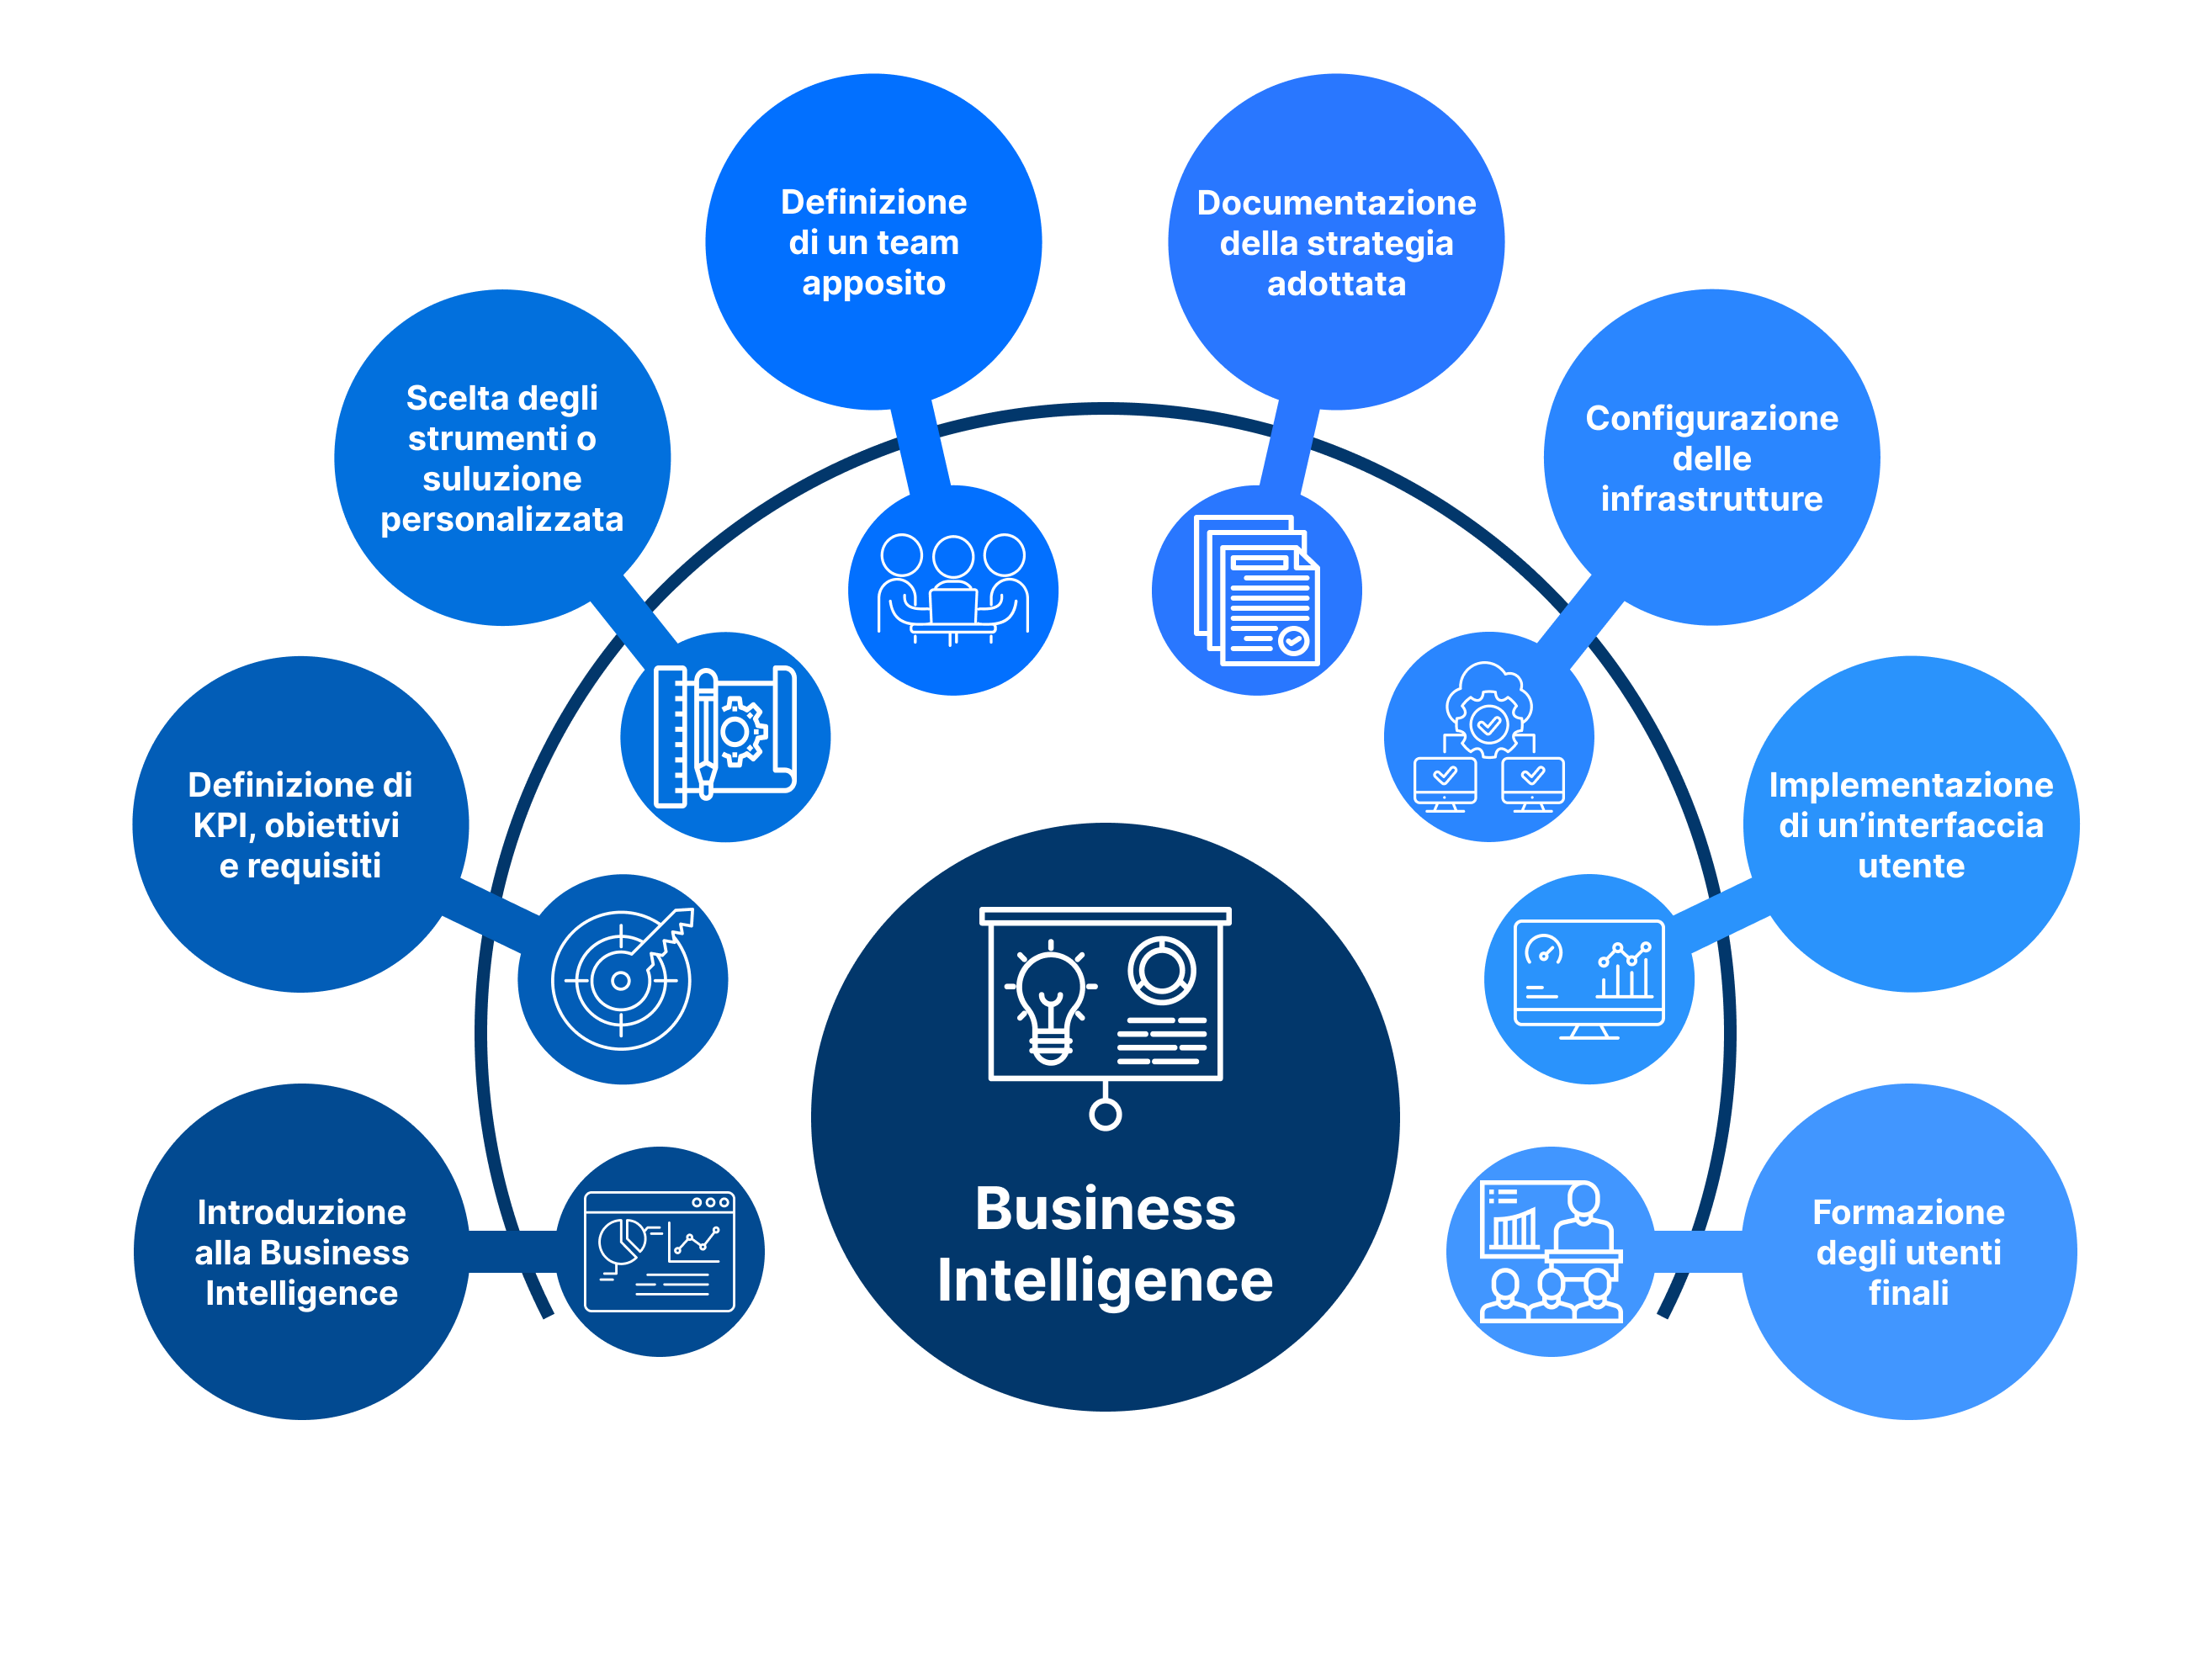
\includegraphics[width=0.75\linewidth]{figure//capitolo_4/Business Intelligence Process.png}
    \caption{Processo di adozione di un sistema di Business Intelligence}
    \label{fig:enter-labelBusiness Intelligence Process}
\end{figure}
\end{comment}

\subsection{Le capacità della BI}

Le capacità della Business Intelligence sono competenze fondamentali che aiutano le aziende a migliorare la propria attitudine all'adattamento al cambiamento e all'esecuzione. Per quanto siano molte le ricerche a riguardo, è rimasto in gran parte silente il ruolo delle capacità della BI nel raggiungere l'adeguato abbinamento tra la BI e l'ambiente decisionale in cui è implementata.
Di seguito sono riportate le capacità prima accennate:\cite{bi_capabilities}

\begin{itemize}
    \item \textit{Qualità dei dati}. La BI si basa principalmente sui dati numerici, che vengono analizzati, gestiti e misurati. Proprio per questo motivo la qualità dei dati è un requisito fondamentale ed imprescindibile in questo mondo. Quando si parla di qualità dei dati si intende che essi siano consistenti e completi, perché diversamente non avrebbero una grossa affidabilità.
    \item \textit{Integrazione con altri sistemi}. Poiché il sistema di BI dipende da altri sistemi, un'importante caratteristica è la sua capacità di interoperabilità con questi. In questo caso, quando si parla di integrazione, si intende sia in ambito software che in ambito hardware.
    \item \textit{Accesso per gli utenti}. Dato che i sistemi di BI non hanno un solo utilizzo, obiettivo o scopo, non è possibile creare una soluzione onnicomprensiva adattabile a tutti i problemi. Per questo motivo è congeniale mettere a disposizione di utenti diversi gli strumenti di BI, in modo che questi possano creare i propri report e svolgere le relative analisi in totale autonomia senza alcuna difficoltà.
    \item \textit{Flessibilità}. Per far sì che una soluzione sia ottimale, è necessario che questa si adatti alle necessità e all'evoluzione dei dati e dell'organizzazione stessa (tecnologie e normative da dover applicare).
    \item \textit{Supporto alla gestione del rischio}. La gestione del rischio permette di aiutare nella presa di decisioni in condizioni spesso incerte. Questa capacità è cruciale per le organizzazioni che operano in ambienti ad alto rischio. Poiché nonostante esistano rischi e instabilità in ogni decisione aziendale, le compagnie cercano di adottare qualsiasi sistema che possa diminuire tale rischio, e la BI è uno di questi.
\end{itemize}

\subsection{BPI}

La progettazione dei processi e le tecnologie di automazione vengono sempre più utilizzate dalle aziende che cercano di migliorare le qualità e l'efficienza dei loro processi amministrativi e produttivi e fornire rapidamente e in modo affidabile servizi alle aziende e ai clienti individuali. Per svolgere queste attività al meglio, sono molte le aziende che decidono di adottare delle soluzioni che prendono il nome di \textbf{Business Process intelligence} (\textit{BPI}). Con questo termine si fa riferimento all'applicazione di tecniche di BI per lo sviluppo e l'implementazione di processi aziendali e comprende molte ambiti di applicazione (ad esempio, monitoraggio, analisi e scoperta dei processi, controllo di conformità, operazioni di previsione ed ottimizzazione), ovvero nell'ambito della \textit{BPM}\footnote{Il \textit{Business Process Management} (\textit{BPM}) è una disciplina che adotta diversi metodi per scoprire, modellare, analizzare, misurare, migliorare e ottimizzare i processi aziendali\cite{gartner_bpm}}.\cite{academiaedu_bpi_definition}

\begin{comment}
\begin{figure}
    \centering
    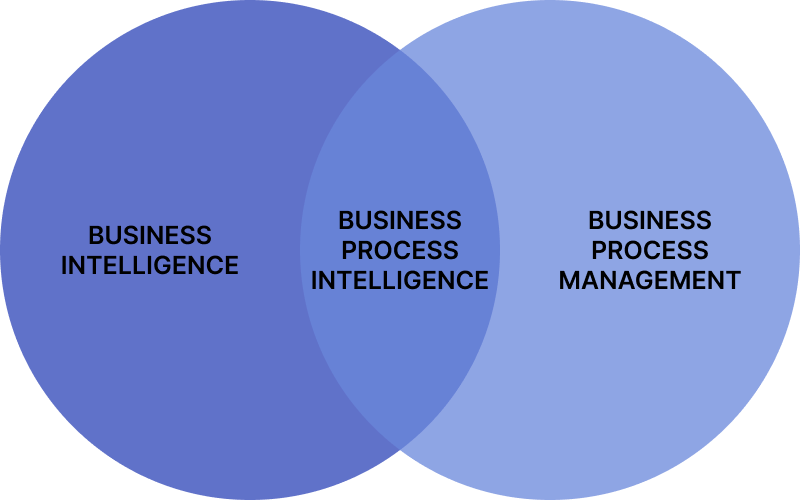
\includegraphics[width=0.5\linewidth]{figure//capitolo_4/Business Process Intelligence.png}
    \caption{La Business Process Intelligence}
    \label{fig:Business Process Intelligence}
\end{figure}
\end{comment}

Date le molteplici possibilità e l'elevato spettro di applicazione, la business process intelligence dispone di diverse funzionalità che offrono altrettanti livelli di automazione per la gestione della qualità dei processi, ovvero:\cite{academiaedu_bpi_feautures}

\begin{itemize}
    \item \textit{Analisi}. La BPI permette agli utenti di analizzare le esecuzioni dei processi completati sia dal punto di vista aziendale che da quello programmatico per gli operatori IT. Inoltre, non solo offre molti sistemi di reportistica, ma la BPI permette anche di analizzare la progettazione di un modello di processo e identificare le tecniche per poterlo migliorare.
    \item \textit{Predizione}. La BPI permette di applicare modelli predittivi ai processi in esecuzione in modo da poter identificare preventivamente la possibilità di riscontrare eccezioni o comportamenti imprevisti e indesiderati. Anche in questo caso, è possibile avere un punto di vista aziendale oppure programmatico.
    \item \textit{Monitoraggio}. La BPI può monitorare ed analizzare le istanze dei processi che sono in esecuzione e informare l'utente nel caso vengano riscontrate situazioni insolite. Grazie a ciò, un utente può visualizzare e analizzare lo stato attuale del sistema, dei processi, dei servizi e delle risorse attualmente in uso e attività. Inoltre, con determinati principi di automazione, è possibile svolgere azioni predefinite in caso di situazioni critiche.
    \item \textit{Controllo}. La BPI, sfruttando il monitoraggio e la predizione dei processi, può interagire con il \textit{BPMS} (\textit{Business Process Management System}) per evitare delle degradazioni di qualità previste ed effettive.
    \item \textit{Ottimizzazione}. La BPI può individuare delle possibili aree di miglioramento nelle definizioni dei processi aziendali attualmente in uso e nell'assegnazione delle risorse ai relativi servizi in attività. Ciò permette una possibile diminuzione dei costi e un aumento dell'efficienza dei processi.
\end{itemize}

% TODO: Immagine feature BPI (?)

% TODO: Aggiungere? \subsection{Possibili soluzioni - tipologie di BI}
% TODO: Aggiungere? \subsection{La BI adattiva}
% TODO: Aggiungere? \subsection{I ruoli in un sistema di BI}

\subsection{La Business Analytics}

Oltre alla Business Intelligence, per quanto meno conosciuta, esiste anche la \textbf{Business Analytics} (\textbf{BA}) che comprende soluzioni adottate per definire modelli di analisi e simulazioni per creare scenari, comprendere realtà e prevedere possibili future situazioni. La BA include strumenti di data mining, analisi predittiva, analisi approfondita e statistica per essere fornita come un sistema di utilità per un'utente aziendale.\cite{gartner_ba}

A primo impatto la Business Analytics può sembrare identica alla Business Intelligence, ed effettivamente sono molto simili tra loro, tuttavia esiste una differenza minima quanto sostanziale, ovvero l'adozione dell'analisi predittiva con l'obiettivo di comprendere possibili eventi futuri. In altre parole, sia la BI che la BA sfruttano i dati di eventi e azioni passate ma lo fanno con scopi differenti: la prima focalizza il proprio obiettivo sul comprendere cosa sia accaduto in passato, mentre la seconda focalizza il proprio obiettivo sul comprendere come agire in futuro.\cite{talend_bi_vs_ba} 


\subsubsection{Differenze tra BI e BA}
Per essere più precisi, è possibile affermare che la Business Intelligence adotta l'\textbf{analisi retrospettiva} (\textit{analisi diagnostica} e \textit{analisi descrittiva}), mentre la Business Analytics adotta l'\textbf{analisi prospettiva} (\textit{analisi prescrittiva} e \textit{analisi predittiva}).\cite{researchgate_bi_and_ba_analytics}

Per comprendere meglio le differenze tra le due tipologie di analisi, di seguito è riportata una tabella riepilogativa:\cite{knowledgehut_bi_vs_ba}

\begin{comment}
\begin{table}
    \centering
    \begin{tabular}{ccc}
        Parametri & Business Intelligence & Business Analytics\\
        Definizione & 
        La BI riguarda la comprensione del passato e del presente di un'azienda.& La BA riguarda la previsione dei risultati futuri delle azioni intraprese dall'azienda.\\
        Focus & 
        Gli strumenti di BI si concentrano sulla gestione dei dati.& 
        Gli strumenti di BA si concentrano sull'analisi dei dati.\\
        Applicazioni & 
        Gli strumenti di BI sono progettati per fornire informazioni dettagliate sulle prestazioni della tua azienda nel tempo.&
        Gli strumenti di BA sono progettati per aiutare a prendere decisioni migliori su come ottimizzare le operazioni per il futuro.\\
        Approccio & 
        La BI si concentra sull'analisi diagnostica e sull'analisi descrittiva.& 
        La BA si concentra sull'analisi predittiva e sull'analisi prescrittiva.\\
        Utilizzo & 
        La BI si concentra in genere sul reporting a livello aziendale tra più dipartimenti e team.& 
        La BA in genere si concentra sull'analisi dettagliata di aree specifiche all'interno di un'organizzazione (ad esempio come il marketing).\\
    \end{tabular}
    \caption{Differenze tra Business Intelligence e Business Analytics}
    \label{tab:BI vs BA}
\end{table}
\end{comment}